% !TEX root = ../TechProject.tex

\graphicspath{{Chapter3/}}

\chapter{Machine Learning used for DJing}

\begin{figure}[H]
	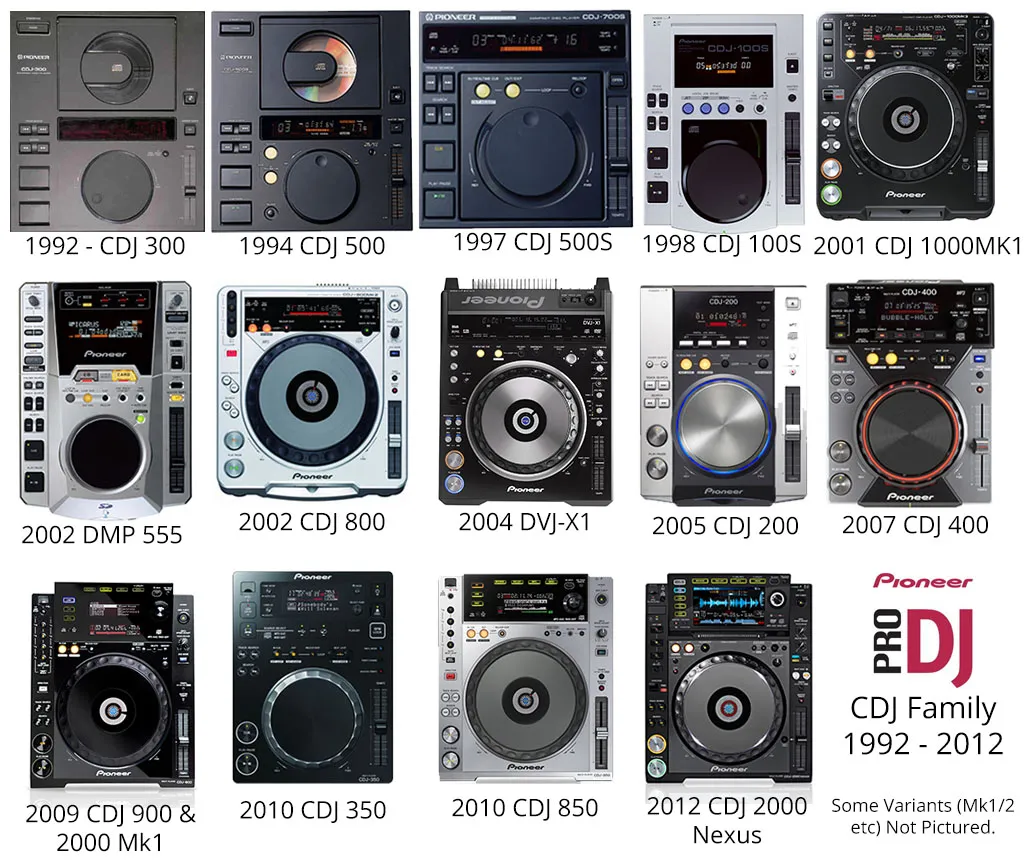
\includegraphics[scale=0.3]{images/pioneers_history}
	\centering
	\caption{Pioneer CDJ models from 1992-2012 \citep{chesters_history_2017}} 
\end{figure}

This chapter answers the following research question:
\\

\textit{Is the proposed method a suitable solution for the automated recommendation of songs suitable for adding to a given DJ set?} 
\\
\\
DJing is a practice that has been the backbone of many sub cultures since the late 60s \citep{brewster_last_2014}. DJing has contributed to the evolution of various genres like Disco, Reggae, and the many forms of electronic dance music \citep{partridge_dub_2010} \citep{reynolds_energy_2013}. DJing traditionally involves two turntables and to transition from one song to another in a stylised or fluid manner. As the rise of digital audio happened within the 1990s saw the creation of CDJ's, and with it the introduction of mixing tool software's such as Pioneers rekordbox. Mixing tool software's makes use of music information retrieval techniques to lower the difficulty of organising and preparing for a DJ set \citep{kim_automatic_2017}. 


Music Information Retrieval is based on finding and compartmentalising the various aspects of music, including rhythm, timbre and melody \citep{orio_music_2006}. Different implementations of music information retrieval varies from source separation and beat tracking. These tasks involve machine learning and deep learning algorithms, and are now fully embedded in DJ software's \citep{rekordbox_rekordbox_2020}. 

\section{Source Separation}

Source separation involves estimating specific sources in one mixed signal. A music based example involves separating an instrument or voice within a track \citep{sgouros_efficient_2022}. Deep learning advancements has helped improve source separation in different fields. An example of this is U-nets, a convolutional neural network that proved effective in segmenting biomedical images \citep{ronneberger_u-net_2015}. With the use of spectrograms, a very similar model was used in a music source separation model \citep{jansson_singing_2017}. Deezer  further adapted this on their popular open source separator Spleeter \citep{hennequin_spleeter_2020}. Despite no published method, popular DJ manufacturer, Serato, released the Serato Stems update to there DJ software which provides similar functionality to Spleeter but in real time \citep{kirn_review_2023}. This has allowed DJs to make remixes in real time, separating instruments or voices from chosen songs.

As with most machine learning models, a rich dataset is essential for an applications accuracy \citep{jain_overview_2020}. The data used trained for Jansson's U-Net model involved 20,000 track pairs of acapella and instrumental tracks \citep{jansson_singing_2017}. These given track pairs are hard to come by in DJ sets so the proposed model could not aid to further developments in source separation.


\section{BPM, key, genre classification}

\begin{figure}[H]
	\hspace*{-1.9cm}
	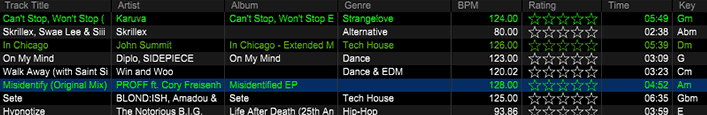
\includegraphics[scale=0.7]{images/rekordbox}
	\centering
	\caption{Playlist in rekordbox showing calculated BPM's and keys \citep{rekordbox_rekordbox_2023}} 
\end{figure}


As mentioned in context based filtering, Audio classification involves retrieving metadata from analysing an audio file \citep{sharma_audio_2021}. Context based filtering show its use for finding similar songs, but audio classification models is also used in DJ software's for calculating tempo, key and other musical attributes.

Despite increased popularity with deep learning, traditional machine learning techniques proves powerful enough for key detection. The Support Vector Machine proposed by George et. al had an accuracy value of 91.49\% and performed better compared to previous papers \citep{george_development_2022}. Support Vector Machine works well due its use of the kernel track and being able to handle linearity and non-linearity in data effectively \citep{hofmann_support_2006}. Having key information is essential within DJing because assuring the keys either match or modulate functionally assures fluidity in the transition. 

With tempo detection, the current state of the art makes use of Temporal Convolutional Networks to estimate the tempo, as well the up and down beat \citep{bock_deconstruct_2020}. The foundation of the model was explored previously \citep{bock_multi-task_2019}, but found that incorporating an extra dilation rate to each layer of the model gave more accurate results. Knowing the tempo of a given song is one of the main draws of CDJs over vinyl turntables, so further developments in tempo detection will inevitably find itself implemented in DJ software's.

As the case for the BPM and key, the advancement of genre classification has had some significant contirbutions in recent years. The most recent signification is a model that uses short-time fourier transform, pitch, timbre and NMF feautres are extracted from a given piece of audio, which is then fed through a deep belief neural network and a Wale Integreated SnO algorithm \citep{kumaraswamy_optimal_2022}. Advancements in genre classification would be helpful within the DJ world as it would help the organisation of playlists for a given DJ.

\section{Automated Mixing}
As well the advances of classification and separation that will aid a DJ, there are an equal amount of advances that could replace them. In February 2023, Spotify began unravelling its brand new DJ feature, combining situational music recommending accompanied by an AI generated host, mimicking the role of a personal broadcast DJ \citep{naomi_spotify_2023}. Within the research world, there have been advances on not just the mimiking of a human DJ's dialogue, but also the way in which a human would transition from one song to the next.

Spotify have some level of implementation to this already and have ran experiments to show a general further appreciation to playlist if it includes DJ-style transitions \citep{bittner_automatic_2017}. Bittners playlist sequencer also included an attempt of DJ-style tranistions, they used peak detection to determine where abouts in the song the "drops" occurs, and gave specific rules to assure appropriate drop in and drop out points for a given track \citep{bittner_automatic_2017}.  However there means of working out up and down beat was ineffective and greatly effected the fluidity of the transitions. A recent attempt at just the transition aspect of this found that using Boykov-Kolmogorov algorithm alongside spectrogram analysis of the two given songs made for great results for songs with similar tempos and keys \citep{robinson_automated_2023}.

\section{Summary}
\textbf{\textit{Write a summary}}

% note that \Blindocument has 5 numbered levels, despite setting secnumdepth above. I (and many style guides) would suggest using no more than 3 numbered levels (incl. the chapter), with the option of a fourth unnumbered level.